% \chapter{Review on GCN}

\section{Introduction}

The primary work of the paper is based on the findings of T. M. Kipf and M. Welling, 
who invented measures for classification in graph network. 

Graph network classification is different from original graphical classification in that graphical data is mostly pixels or matrix which lines up into Euclidean Structure. Original classification models, such as the Convolution Neutral Network, apply convolution operators on the Euclidean Structure to substract features from pixels, as shown in Figure \ref{cnn-illustration}.

\begin{figure}[H]
    \centering
    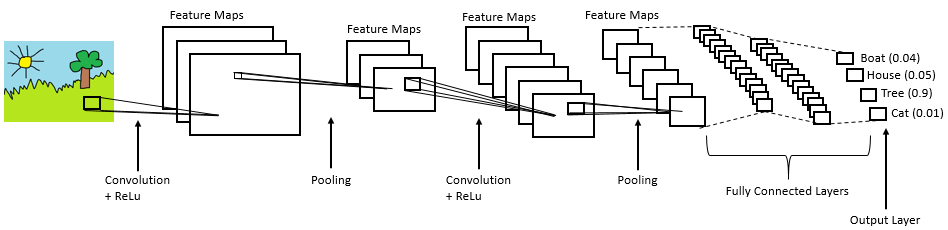
\includegraphics[width=.8\textwidth]{figures/cnn-illustration.png}
    \caption{Convolution on pixels in CNN}
    \label{cnn-illustration}
\end{figure}

\section{Fourier Transformation and Graph Convolution}

While graph data consists of node features and edge features, which are non-Euclidean Structure, the original convolution cannot apply on the data. In the work T. M. Kipf and M. Welling, the covolution operators are re-applied through different methods. The spectral graph theory provides fourier transformation and inverse fourier transformation, given discrete graph adjacency matrix $A$.

\begin{equation}
    \hat{f} = U^T f
    \label{discrete-fourier-transformation}
\end{equation}
    
\begin{equation}
    f = U \hat{f}
    \label{discrete-inverse-fourier-transformation}
\end{equation}

where $U$ is the eigenvector matrix in normalized symmetry graph Laplacian

\begin{equation}
    L = I_N - D^{-\frac{1}{2}}AD^{-\frac{1}{2}} = U\Lambda U^T
    \label{normalized-sysmetry-graph-laplacian}
\end{equation}

The character of fourier tranformation brings sound transformation between convolution operators and fourier operators in non-Euclidean field. 

\begin{equation}
    \begin{aligned}
        \mathcal{F} (h \ast f) & = \mathcal{F} (h) \cdot \mathcal{F} (f) \\
        (h \ast f)_G & = U\left(U^T(h)\odot U^T(f)\right) \\
    \end{aligned}
    \label{graph-convolution}
\end{equation}

where $\odot$ is the Hadamard Product. 

The calculation of graph convolution can be simplified throught the work of Hammond et al. on \textit{Wavelets on Graphs via Spectral Graph Theory}\cite{Hammond2009WaveletsOG}, gaining Equation \ref{approximated-graph-convolution}.

\begin{equation}
    (h \ast f)_{G'} = \sum _ {k=0} ^ K h' _ k T _ k (\tilde{L}) x
    \label{approximated-graph-convolution}
\end{equation}

where $T_k (x)$ denotes the $k$th Chebyshev polynomials, $h'$'s denote the Chebyshev coefficient vectors, $\tilde{L} = \frac{2}{\lambda_{max}}L - I_N$, $\lambda_{max}$ denotes the maximum eigenvalues of $L$, the normalized symmetry Laplacian. The detailed exploration should refer to work of Kipf et al.\cite{DBLP:journals/corr/KipfW16}
